\documentclass{article}
\usepackage{graphicx} % Required for inserting images
\usepackage{geometry}
\usepackage{circuitikz}
\usepackage{siunitx}
\usepackage{CJKutf8}
\usepackage{amsmath}
\usepackage{amssymb}
\usepackage{caption}
\usepackage{float}
\usepackage{subcaption}
\geometry{top=10mm, left=20mm, a4paper}
\title{Feddback Circuit Active Filter Report}
\author{梁程捷(B11901136),吳奕娃(B11901080)}
\date{}

\begin{document}
\begin{CJK*}{UTF8}{bkai}
\maketitle

%============Differential Amplifier====================
\section*{Band Pass Filter}
\begin{minipage}{0.5\textwidth}
\begin{table}[H]
\begin{tabular}{|c|c|c||c|c|c|}
    \hline
    $f$ (\unit{\kilo\hertz}) &  $V_i$ (V)& $V_o$ (V) & $f$ (\unit{\hertz}) &  $V_i$ (V)& $V_o$ (V)\\
    \hline\hline
    0.5	    & 2.040 & 0.12 & 15     & 0.360 & 1.32   \\
    1       & 2.060 & 0.22 & 18     & 0.360 & 1.20  \\
    2	    & 2.040 & 0.42 & 19     & 0.560 & 1.70  \\
    3	    & 2.040 & 0.63 & 20     & 0.560 & 1.52   \\
    5	    & 1.640 & 1.08 & 20.5   & 0.490 & 1.24   \\
    10	    & 0.940 & 1.58 & 21     & 0.560 & 1.36   \\
    12	    & 0.340 & 0.86 & 25     & 0.540 & 0.96   \\
    12.5	& 0.480 & 1.30 & 30     & 0.540 & 0.74   \\
    13      & 0.340 & 1.02 & 40     & 0.480 & 0.52   \\
    14      & 0.340 & 1.18 &        &       &        \\
\hline
\end{tabular}
\caption{raw experimental data}
\end{table}
\end{minipage}\hspace{20mm}
\begin{minipage}{0.5\textwidth}
    \begin{figure}[H]    
        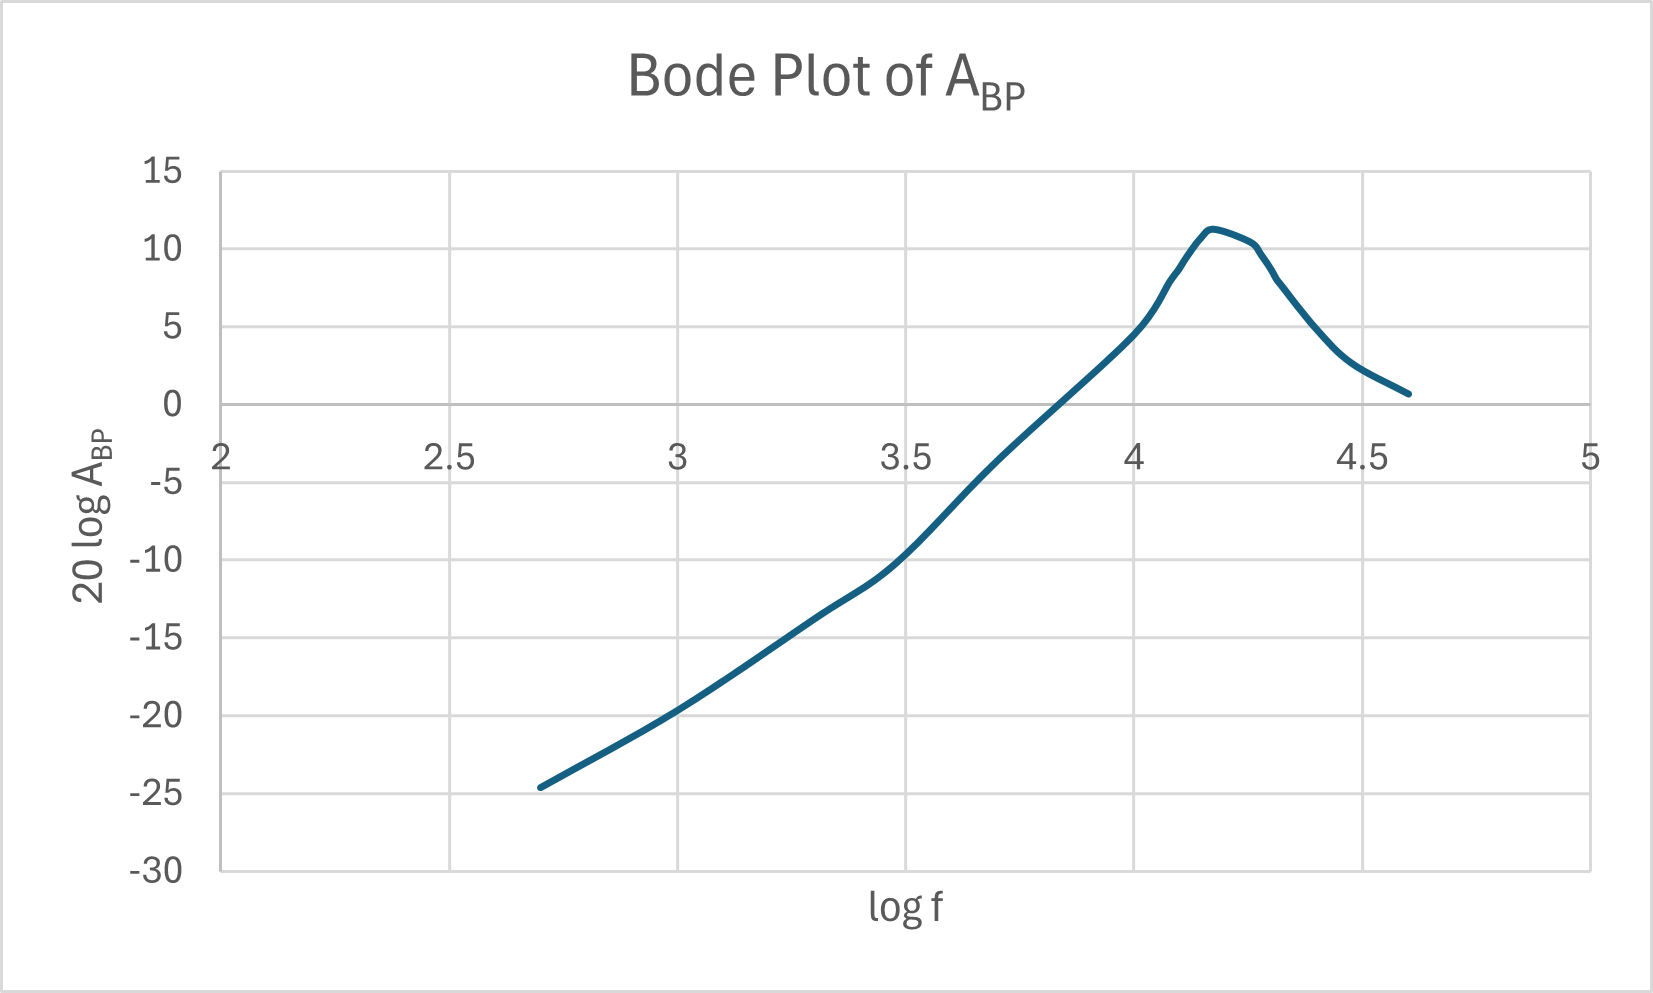
\includegraphics[scale=0.55]{Abp_bode_plot.png}
        \caption{Bode Plot of $A_{BP}$}
    \end{figure}
\end{minipage}
\vspace{3mm}
\textbf{Midband gain $A_{max} = \frac{1.24}{0.4}$ = 3.1 V/V}, \textbf{$f_{3dB}$ = 365 \unit{\kilo\hertz}}

\section*{Reflections}
\subsection*{梁程捷}
這次實驗我們兩個電路都有做,differential amplifier最後的結果發現是low pass,不是band pass,因爲沒有耦合的大電容,就跟課程一樣。
\subsection*{吳奕娃}
這次的實驗做得還算順利,唯一比較麻煩的地方是在第一個實驗,做低頻率的時候示波器上的訊號不太穩,造成量取數值上的困難。
\end{CJK*}
\end{document}
